%!TEX encoding = IsoLatin

%% Document is article 
\documentclass[a4paper]{article}

%% ----------------------------------------------------- PACKAGES ----------------------------------------------------- %%
\usepackage{coolArticle}
\usepackage{algorithm2e}


%% ---------------------------------------------------- DOCUMENT ---------------------------------------------------- %%
\begin{document}

	\titlebox{0.4}{Reinforcement Learning}{Elementary Solution Methods}
	
		
	\vhrulefill{2pt}
	
	\tableofcontents
	
	\vhrulefill{2pt}
	
	\section{Dynamic Programing}
	{
		\paragraph{} Dynamic programing (DP) is a mathematically well-developed theory. It though requires a complete and accurate model of the environment. It entails the basis for every other methods, who attempt to realize the as DP, with lesser computational costs. 
		
		\paragraph{} We hereinafter assume that the state space and each state's space action is finite (i.e $\vert \mathcal{S} \vert <\infty$ and $\forall{s}\in\mathcal{S}, \, \vert \mathcal{A}(s)\vert < \infty$). The dynamic is supposed to be fully given by the set of transition probabilities $\mathcal{P}_{ss'}^a, \mathcal{R}_{ss'}^a$ for all state and relative actions. 
		
		\paragraph{} Remember that the optimal state value function $V^*$ and action value function $Q^*$ verify the \textcolor{red}{Bellman optimality equations} : 
		\begin{equation}
			\begin{aligned}
			&\forall{s}\in\mathcal{S}, \quad V^*(s) = \max_{a\in\mathcal{A}(s)} \sum_{s'} \mathcal{P}_{ss'}^a \left[ \mathcal{R}_{ss'}^a + \gamma V^*(s')\right] \\
			&\forall{(s,a)}\in\mathcal{S}\times\mathcal{A}(\mathcal{S}), \quad Q^*(s,a) = \sum_{s'} \mathcal{P}_{ss'}^a \left[ \mathcal{R}_{ss'}^a + \gamma \max_{a'\in\mathcal{A}(s')} Q^*(s',a')\right] 
			\end{aligned}
		\end{equation}
		
		\subsection{Policy evaluation}
		{
			\paragraph{} We hereinbefore describe how to compute the state value function for a policy $\pi$. This is called the \textbf{\textcolor{red}{policy evaluation}} problem, or the \emph{prediction problem}. 
			
			\paragraph{} We have that $\forall s \in\mathcal{S}$ : 
			\begin{equation}
				V^\pi(s) = \sum_{a\in\mathcal{A}(s)} \pi(s,a) \sum_{s'} \mathcal{P}_{ss'}^a \left[ \mathcal{R}_{ss'}^a + \gamma V^\pi(s')\right] 
			\end{equation}
			If the model is known, this gives us $\vert \mathcal{S}\vert $ simultaneous linear equations with $\vert \mathcal{S} \vert $ unknowns. Even if it is analytically solvable, it might result it tedious computations. Therefore iterative methods are more suitable ways of solving this problem. 
			
			\paragraph{} Let $V_0\, : \, S \to \mathbb{R}$ an initial , arbitrary mapping for the state value function. We build the sequence $(V_k)_k$ of mapping using the Bellman equation for $V^\pi$ as an update rule : 
			\begin{equation}
				\forall{s}\in\mathcal{S}, \quad V_{k+1} (s) =  \sum_{a\in\mathcal{A}(s)} \pi(s,a) \sum_{s'} \mathcal{P}_{ss'}^a \left[ \mathcal{R}_{ss'}^a + \gamma V_k(s')\right] 
			\end{equation}
			
			\paragraph{} Indeed, $V^\pi$ is a fixed-point problem for the Bellman equation, and therefore we might have chance to convert towards this fixed-point by using it as an iterative formula. It can actually be proved that under the same hypothesis guaranteeing the existence of $V^\pi$ that : 
			\begin{equation} 
				V_k \underset{k\to\infty}{\longrightarrow} V^\pi
			\end{equation} 
			Such a procedure is known as an \textbf{\textcolor{red}{iterative policy evaluation}}. 
			\vspace{10pt}
			
			\coolbox{black}{\textcolor{blue}{Iterative Policy Evaluation Algorithm}}
			{
				\begin{algorithm}[H]
	 				\SetAlgoLined
					\LinesNumbered
					 \KwIn{Policy $\pi$ to be evaluated}
					Init $V(s) = 0$, $\forall{s}\in\mathcal{S}$. 
					\Begin
					{
						\Repeat{$\Delta < 0$}
						{
							$\Delta \leftarrow 0$ \\
							\ForEach{$s\in\mathcal{S}$}
							{
									$v\leftarrow V(s)$ \\
									$V(s) = \sum_{a\in\mathcal{A}(s)} \pi(s,a) \sum_{s'} \mathcal{P}_{ss'}^a \left[ \mathcal{R}_{ss'}^a + \gamma V(s')\right] $ \\
									$ \Delta = \max{\left(\Delta, \vert v - V(s)\vert \right)}$
							}
						}
					}
 					\KwOut{$V \simeq V^\pi$ state value function for policy $\pi$} 
				\end{algorithm}
			}
			
			\paragraph{} There exist two implementation of this algorithm : one that needs to keep trace of both the old and new iterations on the state-value function estimate, and another that does the actualization \emph{in-place}. The latter is known to converge faster. 
		}
		
		\subsection{Policy improvement}
		{
			\paragraph{} We just saw how to compute the value function of a given policy. This is also going to help us find better ones. We consider the following problem : given $V^\pi$, would it be better or worse to change the policy ? A good way to find out is, at a given state $s\in\mathcal{S}$, to choose an action $a \neq \pi(s)$, switch to the next state and then follow $\pi$. The value of such a behavior is given by : 
			\begin{equation}
				Q^\pi(s,a) = \sum_{s'}\mathcal{P}_{ss'}^a \left[ \mathcal{R}_{ss'}^a + \gamma V^\pi(s')\right]
			\end{equation}
			If such a value is greater than $V\pi(s)$, the new policy defined by \emph{greedily} taking $a$ in state $s$ is better in overall than $\pi$. 
			
			\paragraph{} The latest exemple is a special case of a general result called the \textbf{\textcolor{red}{policy improvement}} theorem. This theorems state the following : 
			\vspace{10pt}
			
			\coolbox{white}{\textcolor{black}{Policy Improvement Theorem}}
			{
				Let $\pi$ and $\pi'$ be two policies such that $\forall s \in\mathcal{S}$ : 
				\begin{equation}
					Q^\pi(s,\pi'(s)) \geq V^\pi(s) 
				\end{equation}
				then $\pi'$ is a better policy than $\pi$, i.e : 
				\begin{equation}
					\forall{s}\in\mathcal{S}, \quad V^{\pi'}(s) = V\pi(s)
				\end{equation}
			}
			
			\paragraph{} We now consider $\pi'$ the \emph{greedy policy} w.r.t to $Q^\pi$ : $\forall{s}\in\mathcal{S}$ : 
			\begin{equation}
				\begin{aligned}
					\pi'(s) &= \underset{a\in\mathcal{A}(s)}{\text{arg max}} \left\{ Q(s,a) \right \} \\
						 &=  \underset{a\in\mathcal{A}(s)}{\text{arg max}} \left\{ \sum_{s'}\mathcal{P}_{ss'}^a\big[ \mathcal{R}_{ss'}^a + \gamma V^\pi(s')\big] \right \} 
				\end{aligned}
			\end{equation}
			What $\pi'$ achieves is to take the action that looks the best in the short term according to $V^\pi$. This lead to a policy that as good as or better as the original policy $\pi$. 
		}
		
		\subsection{Policy iteration}
		{
			\paragraph{} Once a policy $\pi$ has been improved to yield a better policy $\pi'$, we can then compute $V^{pi'}$ and repeat the improvement process : 
			\begin{equation}
				\pi_0 \overset{E}{\longrightarrow} V^{\pi_0} \overset{I}{\longrightarrow} \pi_1 \overset{E}{\longrightarrow} V^{\pi_1} \overset{I}{\longrightarrow} \hdots \overset{I}{\longrightarrow} \pi^*
			\end{equation}
			For finite MDPs, such a procedure converges to an \emph{optimal policy} and optimal value functions in a finite number of iterations. It is called a \textbf{\textcolor{red}{policy iteration}} procedure. 
			\vspace{10pt}
			
			\coolbox{black}{\textcolor{blue}{Policy iteration}}
			{
				\begin{algorithm}[H]
	 				\SetAlgoLined
					\LinesNumbered
					 \textsf{\emph{1.Initialization}} \\
					 	\indent $V(s)$ and $\pi(s)$ arbitrary for all $s\in\mathcal{S}$ \\
					 \BlankLine
					 \BlankLine
					 \textsf{\emph{2. Policy Evalutation}}\\
					 	\Repeat{$\Delta < 0$}
						{
							$\Delta \leftarrow 0$ \\
							\ForEach{$s\in\mathcal{S}$}
							{
									$v\leftarrow V(s)$ \\
									$V(s) = \sum_{a\in\mathcal{A}(s)} \pi(s,a) \sum_{s'} \mathcal{P}_{ss'}^a \left[ \mathcal{R}_{ss'}^a + \gamma V(s')\right] $ \\
									$ \Delta = \max{\left(\Delta, \vert v - V(s)\vert \right)}$
							}
						}
					\BlankLine
					\BlankLine
					\textsf{\emph{3.Policy Improvement}} \\
					policy\_stable $\leftarrow$ true\\
					\ForEach{$s\in\mathcal{S}$}
					{
						$b\leftarrow \pi(s)$\\
						$\pi(s) = \argmax{a\in\mathcal{A}(s)}{\sum_{s'}\mathcal{P}_{ss'}^a\left[\mathcal{R}_{ss'}^a + \gamma V^\pi(s)\right]}$\\
						If $b\neq \pi(s)$, policy\_stable$\leftarrow$false\\
					}
					If policy\_stable, then stop. Else go to 2. 
				\end{algorithm}
			}
			\subsubsection{Value iteration}
			{
				\paragraph{} There is a major drawback to the previous method. Indeed, each iteration requires a full value evaluation step, which can be challenging for large state space. However, they are many steps in the value evaluation routine that won't have any effect on the policy improvement. One can therefore wonder if he must wait for convergence, or just proceed to a few sweeps in value evaluation and then perform a policy improvement step. 
				
				\paragraph{} In the context of policy iteration, one important special case is when the policy evaluation is stoped after only one full state space sweep. This simplified algorithm is called the \textcolor{red}{value iteration} procedure. It performs a simple backup procedure : 
				\begin{equation}
					\forall{s}\in\mathcal{S}, \quad V_{k+1}(s) = \max_{a}\sum_{s'} \mathcal{P}_{ss'}^a\left[\mathcal{R}_{ss'}^a + \gamma V_k(s')\right]
				\end{equation}
				
				\paragraph{} For any arbitrary $V_0$, it can be shown that $V_k\underset{k\to\infty}{\longrightarrow}V^*$ under the same hypothesis that ensure the existence and unicity of $V^*$. As one can notice, it actually uses the \emph{Bellman optimality equation as an update rule} !
			}
			\subsubsection{Asynchronous DP}
			{
				\paragraph{} Even is value iteration is more tractable than the policy iteration method, it still requires many sweeps in the state space, which can be computationally demanding.
				\paragraph{} The in-place asynchronous DP performs back-ups in any order whatsoever. This methods converges as long as it visits all the states. The most extreme form of this method is achieved when only one sweep is performed in state space before policy improvement. It namely allows to focus on a particular set of the state space, that is though relevant for optimality. 
			}
		}
		
		\subsection{Generalized policy iteration}
		{
			\paragraph{} Policy iterations techniques, as different from one another as they may be, carry on the same iterative steps. One make the value function consistent with the policy (\emph{value evaluation}) and the other make the policy greedy with respect to the current value function (\emph{policy improvement}). 
			
			\paragraph{} The generalized policy iterations (GPI) refers to the general idea of interaction between policy evaluation and policy improvement. Almost all reinforcement learning algorithms can be derived from a GPI. 
			\paragraph{} The full GPI formulation and solving is of course much more tractable than the exaustive search. Given a problem with $\vert \mathcal{S} \vert = n$ and $\forall{s}\in\mathcal{S}, \, \vert \mathcal{A}(s) \vert = m$, an exhaustive search would imply comparing $m^n$ different policies. DP giving out a polynomial complexity in $m$ and $n$, it is therefore exponentially better than the exhaustive search ! 
		}
	}
	\newpage
	
	\section{Monte Carlo Methods}
	{
		\paragraph{} Unlike with dynamic programming, we no longer assume complete knowledge of the environment. Monte Carlo methods only require experience of environment interactions, be it from samples of sequences of state, actions and rewards or online simulated experience. 
		
		\paragraph{} We define Monte Carlo methods only for \emph{episodic states}, in order to have well-defined returns. Only at the end of an episode would the policy and its value function updated. 
		
		\paragraph{} As with DP, we'll consider Monte Carlo methods for : 
			\begin{itemize}
				\item policy evaluation 
				\item policy improvement
				\item generalized policy iterations (GPI)
			\end{itemize}
			
		\subsection{Monte Carlo policy evaluation}
		{
			\paragraph{} The basic idea behind Monte Carlo methods is to average the return observed after a visit to a state on many episodes, in order to approach the expected return (i.e what the value function is trying to express !). 
			
			\subsubsection{Vocabulary}
			{
				\paragraph{} Let $s\in\mathcal{S}$, and we wish to evaluate $V^\pi(s)$. Each occurence of the state $s$ is called a \emph{visit}. We distinguish two different based MC methods : 
				\begin{itemize}
					\item The \emph{every-visit} MC method to estimate $V^\pi(s)$ as the average return following the visit of $s$. 
					\item The \emph{first-visit} MC method which averages only over the returns following the first visits to $s$. 
				\end{itemize}
				\paragraph{} Those are two very similar methods that have slightly different properties. Both converges to $V\pi$ as the number of visits builds up to $+\infty$. In the following, we'll focus on the first-visit method. 
			}
			\subsubsection{The FVMC algorithm}
			{
				\paragraph{} We hereinafter describe more precisely the \textcolor{red}{first-visit Monte Carlo} method for policy evaluation. 
				\vspace{10pt}
				
				\coolbox{white}{\textcolor{blue}{First-Visit Monte Carlo Method}}
				{
					\begin{algorithm}[H]
	 				\SetAlgoLined
					\LinesNumbered
					 \textsf{\emph{1.Initialize : }} \\
					 	\Indp\Indp$\pi \, \leftarrow$ policy to be evaluated  \\
						$V\, \leftarrow$ arbitrary state-value function \\
						$ Return(s) \, \leftarrow$  empty list $\forall s \in\mathcal{S}$\\
						\BlankLine
						\Indm\Indm
					\textsf{\emph{2. Repeat}} (for large number of times) \\
					\Indp \Indp a) Generate an episode using $\pi$ \\
						  	  b) For each state $s$ in the episode : \\
							  \Indp \Indp 
							  	$R \leftarrow $ return following the first occurence of $s$ \\
								Append $R$ to returns \\
								$V(s) = average(Return(s))$
				\end{algorithm}
				}
				
				\subsubsection{Monte Carlo estimation of action values}
				{
					\paragraph{} When a model is not available, it is particularly helpful to estimate action values rather than the state values. Indeed, without a model (especially the transition probabilities $\mathcal{P}_{ss'}^a$), one must explicitly estimate the value of each action in order for the values to be useful in suggesting a policy. 
					
					\paragraph{} We therefore wish to estimate $Q^\pi(s,a)$ for all $s\in\mathcal{S}$, $a\in\mathcal{A}(s)$. The philosophy for estimating those values are te same as the every-visit and first-visit MC methods for state value evaluation. \newline
					However, many relevant state/actions may never be visited. Indeed, if $\pi$ is deterministic, following $\pi$ will allow to observe returns only from one of the actions in each state. The MC estimate of other actions will therefore not improve by experience. 
					
					\paragraph{} This problem is a general problem in reinforcement learning and is designated as \emph{maintaining exploration}. They are two different ways to deal with it : 
					\begin{itemize}
						\item The \textcolor{red}{exploring start} method, where we specify the first step of an episode with a specific state-action pair, with each pair having a non-zero probability of being selected at the start. However, it is not a realistic method for real-life interactions. 
						\item The best solution is therefore to consider policies that are stochastic with a non-zero probability for every action, in every state. 
					\end{itemize}
				}
			}
			
			\subsection{Monte Carlo Control}
			{
				\paragraph{} The term control denotes the approximation of optimal policies. We hereinafter consider a Monte Carlo version of the classical policy iteration. Like with DP, we perform alternative steps of policy evaluation and policy improvement (policy evaluation being performed as describe before). 
				
				\begin{equation}
				\pi_0 \overset{E}{\longrightarrow} V^{\pi_0} \overset{I}{\longrightarrow} \pi_1 \overset{E}{\longrightarrow} V^{\pi_1} \overset{I}{\longrightarrow} \hdots \overset{I}{\longrightarrow} \pi^*
			\end{equation}
			
				\paragraph{} We assume that episodes are generated with exploring start and that we observe an infinite number of episodes. Therefore the Monte-Carlo method computes $Q^{\pi_k},\, \forall{k}$ exactly. As before, policy improvement is done by making the policy greedy w.r.t the current value function. With the available action-value function, no model ins needed for constructing the greedy policy : 
				\begin{equation}
					\forall s\in\mathcal{S}, \, \pi(s) = \argmax{a\in\mathcal{A}(s)}{Q^\pi(s,a)}
				\end{equation}
				Hence policy improvement is performed by constructing $\pi_{k+1}$ by making it greedy with respect to $Q^{\pi_k}$. We can show that the \emph{policy improvement} theorem still checks out. Indeed, $\forall{s}\in\mathcal{S}$ : 
				\begin{equation}
					\begin{aligned}
						Q^{\pi_k}(s,\pi_{k+1}(s)) &= Q^{\pi_k}(s,\argmax{a\in\mathcal{A}(s)}{Q^{\pi_k}(s,a)})\\
										      &= \max_{a\in\mathcal{A}(s)} Q^{\pi_k}(s,a)\\
										      &\geq Q^{\pi_k}(s,a) \quad \forall a\in\mathcal{A}(s) \\	
										      &\geq Q^{\pi_k}(s,\pi_k(s))\\
										      & \geq V^{\pi_k}
					\end{aligned}
				\end{equation}
				which ensures that each $\pi_{k+1}$ is uniformly better that $\pi_k$ (unless it is equal to $\pi_k$, in which case both policies are optimal). 
				
				\paragraph{} However, we've made two unlikely assumptions to achieve this result : exploring start and infinite number of episodes. Like we did in DP, the latest can be discarded, as we do not need full convergence of the value evaluation process to perform policy improvement. Like with some extreme case of the GPI, is would be natural for MCPI to alternate bewteen evaluation and improvement on an episode-to-episode basis. This leads to the \emph{Monte Carlo with Exploring Starts} policy iteration algorithm. This algorithms ensures that if it converges, it must converges toward an optimal policy. However, convergences has not yet been formally proven, and remains an open question in the reinforcement learning community. 
				
				\subsubsection{On Policy Monte Carlo Control}
				{
					\paragraph{} As said before, we need to find a way to avoid the unlikely assumption of exploring start. Therefore we need to find a way to ensure that all actions are selected infinitely often. The first approach in doing that is called on-policy control (it evaluates and improve directly the policy that is used to make the decisions). 
					
					\paragraph{} For on-policy MC control, the policy is assumed to be \textbf{\textcolor{red}{soft}} : 
					\begin{equation}
						 \forall (s,a)\in\mathcal{S}\times \mathcal{A}(s), \quad \pi(s,a) > 0, 
					\end{equation}
					To improve the policy, we gradually shift the policy toward the soft-equivalent of greediness, which we denote as $\varepsilon$-greedy. \newline
					For the $\varepsilon$-greedy policy, the optimal value is selected with $1 - \varepsilon$ probablity, and a random action is taken with $\varepsilon$ probability. Such a policy is still soft, since : 
					\begin{equation}
						 \forall (s,a)\in\mathcal{S}\times \mathcal{A}(s), \quad \pi(s,a) \geq \frac{\varepsilon}{\vert \mathcal{A}(s) \vert } > 0
					\end{equation}
					We saw that without the exploring start hypothesis, we cannot improve the policy by making it greedy with respect to the action-value function. Fortunately, the GPI does not need for us to take it all the way to greediness. Actually, the $\varepsilon$-greedy policy, with respect to $Q^\pi$ is an improvement over any $\varepsilon$-soft policy. Indeed, $\forall s \in\mathcal{S}$ :
					\begin{equation}
						\begin{aligned}
							Q^\pi(s,\pi'(s)) &= \sum_{a\in\mathcal{A}(s)} \pi'(s,a)Q^\pi(s,a)\\
									       &= (1-\varepsilon)\max_a Q^\pi(s,a) + \frac{\varepsilon}{\vert \mathcal{A}(s) \vert }\sum_{a\in\mathcal{A}(s)} Q^\pi(s,a) \\
									       &\geq \frac{\varepsilon}{\vert \mathcal{A}(s) \vert }\sum_{a\in\mathcal{A}(s)} Q^\pi(s,a) + (1-\varepsilon)\sum_{a\in\mathcal{A}(s)} \frac{\pi(s,a) - \frac{\varepsilon}{\vert \mathcal{A}(s)\vert }}{1 - \varepsilon}Q^\pi(s,a) \\
									       &\geq \sum_{a\in\mathcal{A}(s)} \pi(s,a)Q^\pi(s,a) = V^\pi(s)
						\end{aligned}
					\end{equation}
					thus $\pi' \geq \pi$, with equality holding for $\pi'$ and $\pi$ being optimal among the $\varepsilon$-soft policies. 
					
					\vspace{10pt}
					
					\coolbox{white}{\textcolor{blue}{$\varepsilon$-soft On-Policy Monte Carlo Control Algorithm}}
					{
					\begin{algorithm}[H]
	 					\SetAlgoLined
						\LinesNumbered
						 \textsf{\emph{1.Initialize }} for all $s\in\mathcal{S}$, $a\in\mathcal{A}(s)$ : \\
						 	\Indp \Indp
								$ Q(s,a) \leftarrow $ arbitrary \\
								$Return(s,a) \leftarrow$ empty list \\
								$\pi \leftarrow$ arbitrary $\varepsilon$-soft policy
								
							\Indm \Indm 
					 		\BlankLine
							\BlankLine
							\textsf{\emph{2.Repeat Forever }} \\
							\Indp \Indp 
								(a) Generate an episode using $\pi$ \\
								(b) For each pair $(s,a)$ in that episode :\\
								\Indp \Indp 
									$R \leftarrow$ return following the occurence of $(s,a)$ \\
									Append $R$ to $Return(s,a)$\\
									$Q(s,a) \leftarrow \text{average}(Return(s,a))$
									
								\Indm \Indm
								
								(c) For each $s$ in the episode : 
								\Indp \Indp 
									$a^* \leftarrow \argmax{a}{Q(s,a)}$ \\
									Forall $a\in\mathcal{A}(s)$ : 
									$$
										\pi(s,a) \leftarrow \left\{ \begin{aligned} 
															&1 - \varepsilon + \frac{\varepsilon}{\vert \mathcal{A}(s) \vert } \text{ if } a=a^*\\
															&\varepsilon \text{ otherwise} 
														\end{aligned}\right. $$
								
								\Indm \Indm 
							
							\Indm \Indm
					\end{algorithm}
					}
					
					\subsubsection{Evaluation a policy while following another}
					{
						\paragraph{} Let's consider the following problem : we have episodes generated from a policy differenet that the one we wish to evaluate. How can we learn $V^\pi$ and $Q^\pi$ with episodes generated with $\pi'$, i.e learn from experience "off" policy ? 
						
						\paragraph{} Of course, we must require that every action taken under $\pi$ is also taken under $\pi'$ : 
						\begin{equation}
							\forall{(s,a)}\in\mathcal{S}\times\mathcal{A}(s), \quad \pi(s,a) >0 \Rightarrow \pi'(s,a)>0
						\end{equation}
						Let us consider the $i$\textsuperscript{th} first visit to some state $s\in\mathcal{S}$. Let $p_i(s)$ and $p_i'(s)$ the probabilities of the sequence that followed that visit under $\pi$ nad $\pi'$. Let $R_i(s)$ be the corresponding return from state $s$. To average these to obtain an unbiased estimate of $V^\pi$, we need only weight them by $\frac{p_i(s)}{p_i'(s)}$, i.e 
						\begin{equation}
							V^\pi(s) \simeq \frac{\displaystyle \sum_{i=1}^{n_s}\frac{p_i(s)}{p_i'(s)}R_i(s) }{\displaystyle\sum_{i=1}^{n_s}\frac{p_i(s)}{p_i'(s)}}
						\end{equation}
						where $n_s$ denoted the number of returns obtained from $s$. 
						
						\paragraph{} At first glance, one can think than the need for $p_i$ and $p_i'$ requires a model of the environment. This is true, but the fact that we only need the ratio of those two quantities bypasses the need of a model : 
						\begin{equation}
							\begin{aligned}
								\forall s\in\mathcal{S}, \quad 
									\frac{p_i(s)}{p_i'(s)} &=\frac{ \prod_{k=1}^{T_{i}} \pi(s_k,a_k)\mathcal{P}_{s_{k}s_{k+1}}^{a_{k}}}{\prod_{k=1}^{T_{i}} \pi'(s_k,a_k)\mathcal{P}_{s_{k}s_{k+1}}^{a_{k}}}\\
									&= \prod_{k=1}^{T_i} \frac{\pi(s_k,a_k)}{\pi'(s_k,a_k)}
							\end{aligned}
						\end{equation}
					}
					
					\subsubsection{Off-Policy Monte Carlo Control}
					{
						\paragraph{} The \textbf{\textcolor{red}{off-policy}} MC control method uses two policies : 
						\begin{itemize}
							\item A policy to generate behavior (\emph{behavior policy})
							\item A policy to be evaluated and improved (\emph{evaluated policy})
						\end{itemize}
						
						\paragraph{} For exploring all possibilities, we recquire the behavior policy to be soft. Therefore, $\pi'$ is maintenant an arbitrary soft policy. 
						\vspace{10pt}
						
						\coolbox{white}{\textcolor{blue}{An off-policy Monte Carlo Control algorithm}}
						{
						\begin{algorithm}[H]
	 					\SetAlgoLined
						\LinesNumbered
						 \textsf{\emph{1.Initialize }} for all $s\in\mathcal{S}$, $a\in\mathcal{A}(s)$ : \\
						 	\Indp \Indp
								$ Q(s,a) \leftarrow $ arbitrary \\
								$ N(s,a) \leftarrow 0$ \\
								$ D(s,a) \leftarrow 0$ \\
								$\pi \leftarrow$ arbitrary deterministic policy \\
								
							\Indm \Indm 
					 		\BlankLine
							\BlankLine
							\textsf{\emph{2.Repeat Forever }} \\
							\Indp \Indp 
								(a) Select a policy $\pi'$ and use it to generate an episode: 
								$$ s_0, a_0,r_1 \hdots, s_{T-1}, a_{T-1}, r_T, s_T $$
								(b) $\tau \leftarrow$ latest time at which $a_\tau \neq \pi(s_\tau)$ \\
								(c) For each pair $s$ appearing in the episode at time $\tau$ or later : 						\\						
								\Indp \Indp 
								$t\leftarrow$ time of the first occurence of $(s,a)$ such that $t\geq \tau$\\
									$w \leftarrow \prod_{k=t+1}^{T-1}\frac{1}{\pi'(s_k,a_k)}$ \\
									$N(s,a) \leftarrow N(s,a) + wR_t $ \\
									$D(s,a) \leftarrow D(s,a) + w$ \\
									$Q(s,a) \leftarrow \frac{N(s,a)}{D(s,a)}$ 									
									
								\Indm \Indm
								
								(d) For each $s$ \\
								\Indp \Indp 
									$\pi(s) \leftarrow \argmax{a}{Q(s,a)}$
								
								\Indm \Indm 
							
							\Indm \Indm
							\end{algorithm}
						}
					}
				}
			}
			
			\subsection{Brief Summary}
			{
				\paragraph{} Monte Carlo methods learn value function and optimal policies from experience in the form of sample episodes. It has different advantages over the standard DP method : 
				\begin{itemize}
					\item no model of the environment is needed
					\item easier to focus on small subset of the state
				\end{itemize}
				
				\paragraph{} Maintaining sufficient exploration is an issue in MC method of control, since we need to keep exploring the whole state space to average returns. There exists two solution to that problem : using exploring starts or soft-policies. 
				
				\paragraph{} \emph{On-policy} methods are the name given to methods where the agent commits to always exploring and tries to find the best policy that keeps on exploring. On the other hand, \emph{off-policy} methods explore but learns a deterministic optimal policy that may be unrelated to the policy followed. 
				
				\paragraph{} Monte-Carlo methods are recent, and their convergence properties are unclear. Their effectiveness in practice has also little been tested. 
			}
		}
		\newpage
		
		\section{Temporal Differences Methods}
		{
			\paragraph{} Temporal differences (TD) methods can be seen as a combination of DP and MC methods. Like MC, TD can learn from experience without a model of its environment. However, like DP, temporal differences methods update estimates based on other learned estimates : they are therefore said to \emph{bootstrap}. 
			
			\paragraph{} We'll consider here the problems a policy evaluation and control problem (finding an optimal policy). 
			
			\subsection{Temporal differences policy evaluation}
			{
				\subsubsection{The prediction problem with TD}
				{
				\paragraph{} When MC methods wait until the end of an episode to determine how to increment a given $V(s_t)$, temporal differences methods wait only until the next time step. At time $(t+1)$, they immediately form a target and make a useful update using the observed reward and the estimate $V(s_{t+1})$. 
				
				\paragraph{} The simplest temporal difference method, known as TD(0), gives out : 
				\begin{equation}
					\label{eq::td}
					V(s_t) = V(s_t) + \alpha \big [ r_{t+1} + \gamma V(s_{t+1}) - V(s_t)\big]
				\end{equation}
				As one can see, when the target was $R_t$ for Monte Carlo methods, it is $r_{t+1} + \gamma V(s_{t+1})$ for the TD method. Indeed, as we recall, $\forall s \in\mathcal{S}$ : 
				\begin{equation}
					\begin{aligned}
						V^\pi(s) &= \E[\pi]{R_t \vert s_t=s} \\
							     &= \E[\pi]{r_{t+1} + \gamma V^\pi(s_{t+1}) \vert s_t =s }
					\end{aligned}
				\end{equation}
				When MC update rule is taken from the first line of the equality, TD update rule implements the second line. Equation (\ref{eq::td}) can be explain the following way : 
				\begin{equation}
					\underbrace{V(s_t)}_{\text{new value}} = \underbrace{V(s_t)}_{\text{old value}}+ \underbrace{\alpha}_{\text{learning rate}} \big [ \underbrace{\overbrace{r_{t+1}}^{\text{instant reward}} + \overbrace{\gamma}^{\text{discount rate}} \overbrace{V(s_{t+1})}^{\text{estimate of future value}}}_{\text{learned value}} - V(s_t)\big]
				\end{equation}
				
				\paragraph{} TD therefore combines the sampling of MC and the bootstrap of DP. Actually, TD and MC updates are called as \textcolor{red}{sample backups} because they involve looking ahead to a sample successor state, using its value and the reward along the way to compute a back-up value (and therefore are different than the \emph{full back-up} methods implemented in DP). 
				
				\vspace{10pt}
				
				\coolbox{white}{\textcolor{blue}{Temporal Difference Learning for the State Value Estimation}}
				{
					\begin{algorithm}[H]
	 					\SetAlgoLined
						\LinesNumbered
						 \textsf{\emph{1.Initialize }} $V(\cdot)$ arbitrarily, $\pi$ the policy to be evaluated\\
						 \BlankLine 
						 \BlankLine
						\textsf{\emph{2. Repeat}} for every episode : \\
							\Indp \Indp 
								Initialize $s$ \\
								\textsf{\emph{Repeat}} for every step in the episode : \\
								\Indp \Indp 
									$a\leftarrow$ action given by $\pi$ for $s$ \\
									Take action $a$, observe $r$, switch to $s'$ \\
									$V(s) \leftarrow V(s) + \alpha \big [ r_{t+1} + \gamma V(s_{t+1}) - V(s_t)\big]$\\
									$s\leftarrow s'$\\
								\Indm \Indm 
							until $s\in\mathcal{S}^+$. 
							\Indm \Indm 				
					\end{algorithm}
				}
			}				
			\subsubsection{The advantages of TD prediction method}
			{	
				\paragraph{} TD has many advantages : like MC, there is no need for a model for the environment, rewards and next step probability distributions. It is naturally implement \emph{on-line}, in a fully incremental fashion (unlike MC methods, we don't have to wait for an episode to return to perform a value update, which can make the learning slow). Hence, TD methods are particularly efficient for very long episodes, and crucial for \emph{continuing tasks}. 
				
				\paragraph{} However, one may ask if there is still any guarantee of convergence ? The answer is yes. For any fixed policy, the TD algorithm has been proved to converge to $V^\pi$ with probability $1$ if the step size parameter decreases according to the usual stochastic approximation conditions : 
				\begin{equation}
					\sum_k\alpha_k(a)  = +\infty \quad \text{ and } \quad \sum_k\alpha_k^2(a) < + \infty
				\end{equation}
				where $\alpha_k(a)$ is the learning rate for the k\textsuperscript{th} visit of the pair $(s,a)\in\mathcal{S}\times\mathcal{A}(s)$. 
				
				\paragraph{} As to which of the MC or TD method converges faster to the correct value function, it is still an open question in reinforcement learning. However, TD methods have in practice been found to converge faster than MC methods. 
			}
			}
			
			\subsection{Temporal Difference Control}
			{
					\paragraph{} As we did before, we are going to follow the general pattern of GPI, only this time we'll use temporal difference learning methods for the policy evaluation parts. 
					
					\paragraph{} As with MC methods, we face the need to trade-off between exploration and exploitation. Again, the available approaches fall into two main classes : off-policy and on-policy. 
				\subsubsection{SARSA : On-Policy TD Control}
				{
					\paragraph{} We hereinafter present an on-policy control method. As we recall, we are presented with the following sequence : 
					\begin{figure}[h!]
						\begin{center}
							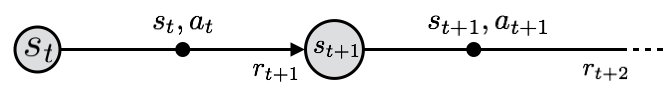
\includegraphics[width=0.5\linewidth]{rl_seq}
						\end{center}
					\end{figure}
					In the previous sections we consider transitions from state to state and learned the values of the states. We now consider transition from state-action pair to state-action pair and learn the action-value function with the following update rule : 
					\begin{equation}
						Q(s_t,a_t) \longleftarrow Q(s_t,a_t) + \alpha\big[ r_{t+1} + \gamma Q(s_{t+1},a_{t+1}) - Q(s_t,a_t) \big]
					\end{equation}
					which is done after every transition from a non-terminal state ( if $s_{t+1}\in\mathcal{S}^+$, then $Q(s_{t+1},a_{t+1}) = 0$). 
					
					\paragraph{} Hence, the update rule uses element of the quintuple event : 
					\begin{equation}
						\big( s_t,a_t, r_{t+1}, s_{t+1}, a_{t+1}\big)
					\end{equation}
					i.e State Action Reward State Action, given it the name \emph{SARSA}. 
					
					\paragraph{} As in all on-policy methods, we continually estimate $Q^\pi$ for the behavior policy $\pi$, and at the same time change $\pi$ toward greediness, with respect to $Q^\pi$.  
					\vspace{10pt}
					
					\coolbox{white}{\textcolor{blue}{The General Sarsa Algorithm}}
					{
						\begin{algorithm}[H]
	 					\SetAlgoLined
						\LinesNumbered
						\emph{\textsf{1. Initialize}} $Q(s,a)$ arbitrarily $\forall (s,a)\in\mathcal{S}\times\mathcal{A}(s)$ \\
						\BlankLine
						\BlankLine
						\emph{\textsf{2. Repeat}} for each episode : \\
						\Indp \Indp 
							Initialize $s$ \\
							Choose $a\in\mathcal{A}(s)$ using a soft policy derived from $Q$ (typically $\varepsilon$-greedy) \\
							Repeat for each step of the current episode :   \\
							\Indp \Indp 
								Take $a$, observe $r,s'$ \\
								Choose $a'$ from $s'$ using policy derived from $Q$ 
								$ Q(s,a) \longleftarrow Q(s,a) + \alpha\big[ r + \gamma Q(s',a') - Q(s,a) \big]$ \\
								$a\leftarrow a'$, $s\leftarrow s' $ \\
								
							\Indm \Indm 
						until $s\in\mathcal{S}^+$.
						\Indm \Indm 
						\end{algorithm}
					}
					
					\paragraph{} The convergences properties of $SARSA$ depend on the nature of the policy's dependency on $Q$. Indeed, $SARSA$ converges with probability $1$ to an optimal policy in action value function as long as all the sate action pars are visited an infinite number of time and the policy converges in the limit to the greedy policy. 
				}
			
				\subsubsection{Q-learning : Off-Policy TD Control}
				{
					\paragraph{} The most important breakthrough in reinforcement learning was the development of an off-policy temporal difference algorithm known as \textcolor{red}{Q-learning}. It's update rule is given by : 
					\begin{equation}
						Q(s_t,a_t) \leftarrow Q(s_t,a_t) + \alpha \big[ r_{t+1} + \gamma \max_{a\in\mathcal{A}(s_{t+1})} Q(s_{t+1},a) - Q(s_t,a_t) \big]
					\end{equation}
					
					\paragraph{} The learned action-value function $Q$ directly approximates $Q^*$, independently of the policy being followed. The policy still has an effect in that it determines which state-actions pairs are visited and updated. However, all that is required for convergence is that all pairs continue to be updated. 
					
					\paragraph{} Along the hypothesis and a variant of the usual stochastic approximation condition on the step-size parameters, $Q_t$ has been shown to converge with probability A to $Q^*$. 
					
					\vspace{10pt}
					
					\coolbox{white}{\textcolor{blue}{Q-Learning Algorithm}}
					{
						\begin{algorithm}[H]
	 					\SetAlgoLined
						\LinesNumbered
						\emph{\textsf{1. Initialize}} $Q(s,a)$ arbitrarily $\forall (s,a)\in\mathcal{S}\times\mathcal{A}(s)$ \\
						\BlankLine
						\BlankLine
						\emph{\textsf{2. Repeat}} for each episode : \\
						\Indp \Indp 
							Initialize $s$ \\
							Repeat for each step of the current episode :   \\
							\Indp \Indp 
								Choose $a\in\mathcal{A}(s)$ using arbitrary policy \\
								Take $a$, observe $r,s'$ \\
								$ Q(s,a) \longleftarrow Q(s,a) + \alpha\big[ r + \gamma \max_{a'\in\mathcal{A}(s')}Q(s',a') - Q(s,a) \big]$ \\
								$s\leftarrow s' $ \\
								
							\Indm \Indm 
						until $s\in\mathcal{S}^+$.
						\Indm \Indm 
						\end{algorithm}
					}
				}
			}			
			\subsection{Brief Summary}
			{
				\paragraph{} Temporal differences methods are the most widely used methods in reinforcement learning. Indeed, they can be applied on line with a minimal amount of computation. 
				
				\paragraph{} The special case of TD methods we displayed hereinbefore should rightly be called \emph{one step, tabular, model-free} temporal difference methods. Indeed, they can be extended to multistep forms, using function approximation rather than tables (giving a link to artificial neural networks). 
			}
		}
	}	
	
\end{document}